
\chapter{Implementing the server logic}
\label{intro} 


\abstract{
The aim of this part of the project was to implement an application that is capable of reacting to different situations that can occur in a smart city. The application should automatically decide, based on the user reason, which forces are needed and also determine which forces are the closest ones. In this project the forces are firefighters, polices and ambulances. In addition to that there are some Hospitals.


The problem to be solved is to register every entity that is driving around in the smart city and monitor their attributes. Especially the users should be monitored, because if they need help the needed forces should be alarmed. Also, it should be possible to update the attributes over time and calculate the distance between the entities.


The problem is solved by differentiate between a registration of an entity or an update of an entity. When an entity is registered a new object with all its attributes is generated and saved in a list. Also, a new communication channel is opened to receive updates for that specific entity. The communication takes place by using the MQTT protocol.


The results of the project were very mixed. The processing of the data did not always work and sometimes led to endless loops. Basic functions like creating entities or calculating the distance all worked perfectly. Under certain circumstances, the system worked as expected and without failures.
}



\section{Introduction}
\label{sec:1}
As part of the interaction concept module, a smart city with various emergency services, a hospital and user vehicles were to be conceptually presented. The project was a group project of the sixth semester in the interaction technology and design course with the aim that all emergency services, hospitals and users can communicate with each other. For example, if a vehicle makes an emergency call, the emergency services that are needed are automatically alerted. 

Figure \ref{overview} shows the communication between the different parts of the project. This chapter describes the processing of the data of the individual vehicles as well as the logic. This is shown in the top left in graphic \ref{overview}. For this, an application should be implemented that meets certain requirements. The requirements and how they were met are explained in more detail in chapter \ref{sec:3}.


\begin{figure}
\sidecaption
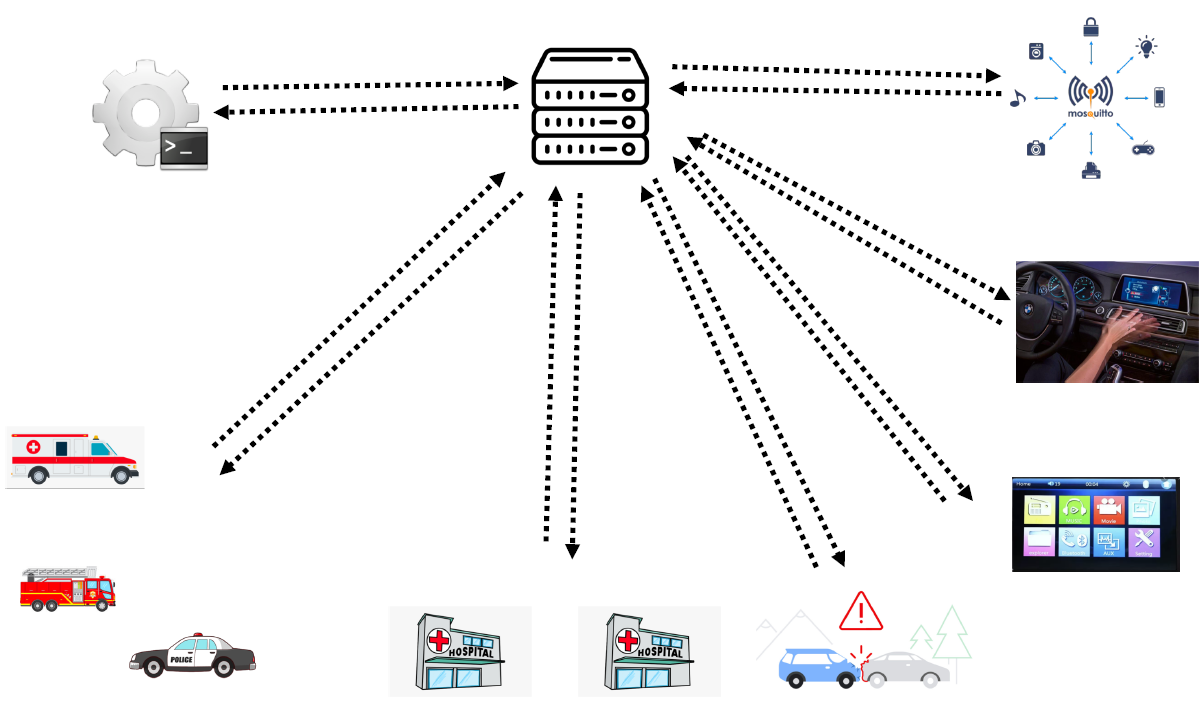
\includegraphics[scale=0.4]{images/walter/uebersicht.png}
\caption{Overview of the project \cite{rettberg_2020}}
\label{overview}
\end{figure}



\section{Related works}
\label{sec:2}

In a practical experiment, an IoT-based system was developed that can observe certain environments such as houses, cities, companies or hospitals. Various environmental variables such as temperature, humidity and pressure were observed. All data was exchanged wirelessly using the MQTT protocol \cite{smartCity}.

Another project that was carried out by the research group Santander built a big data platform for smart cities. The aim of this project was to create a platform that is able to store and use the data that is generated in a city connected by many IoT devices. Another goal of this work is to provide a good example to drive the development of smart cities. 
As part of the project, the so-called CiDAP platform was provided and integrated into an ongoing experimental IoT test field SmartSantander, one of the largest Smart City test fields in the world \cite{santander}.


\section{Proposal (Concept)}
\label{sec:3}

This part of the project was to implement the data processing as well as the logic. Part of the project was that entities can register, and they can also be updated. Communication should take place via the MQTT protocol. The data should be exchanged in .json format. This format lends itself to such an implementation, since it is very robust and can be easily expanded. 

All vehicles that register should be saved in a list provided for them. If a user vehicle makes an emergency call, the emergency services that are available and needed for this type of emergency should be automatically alerted. In addition, the distance of the emergency services to the user should be taken into account, i.e. the emergency services closest to the user are preferably alerted. 

In the event of an accident, a hospital with the right specialist should be chosen. There should be different types of emergency calls, for example for accidents or a heart attack. 

When alerting, the type of emergency call should be given (is it an accident or heart attack), the position of the user at whom he made the emergency call and the distance to the position of the user. This information should be forwarded directly to the alerted vehicles. The user who made the emergency call should get an answer that help is on the way.



The various requirements for the application can be derived from the usecase diagram shown in \ref{usecase}. The extracted requirements are divided into functional requirements, listed in \ref{fr}, and non-functional requirements, which are listed in \ref{nfr}.

\begin{figure}[h]
\sidecaption
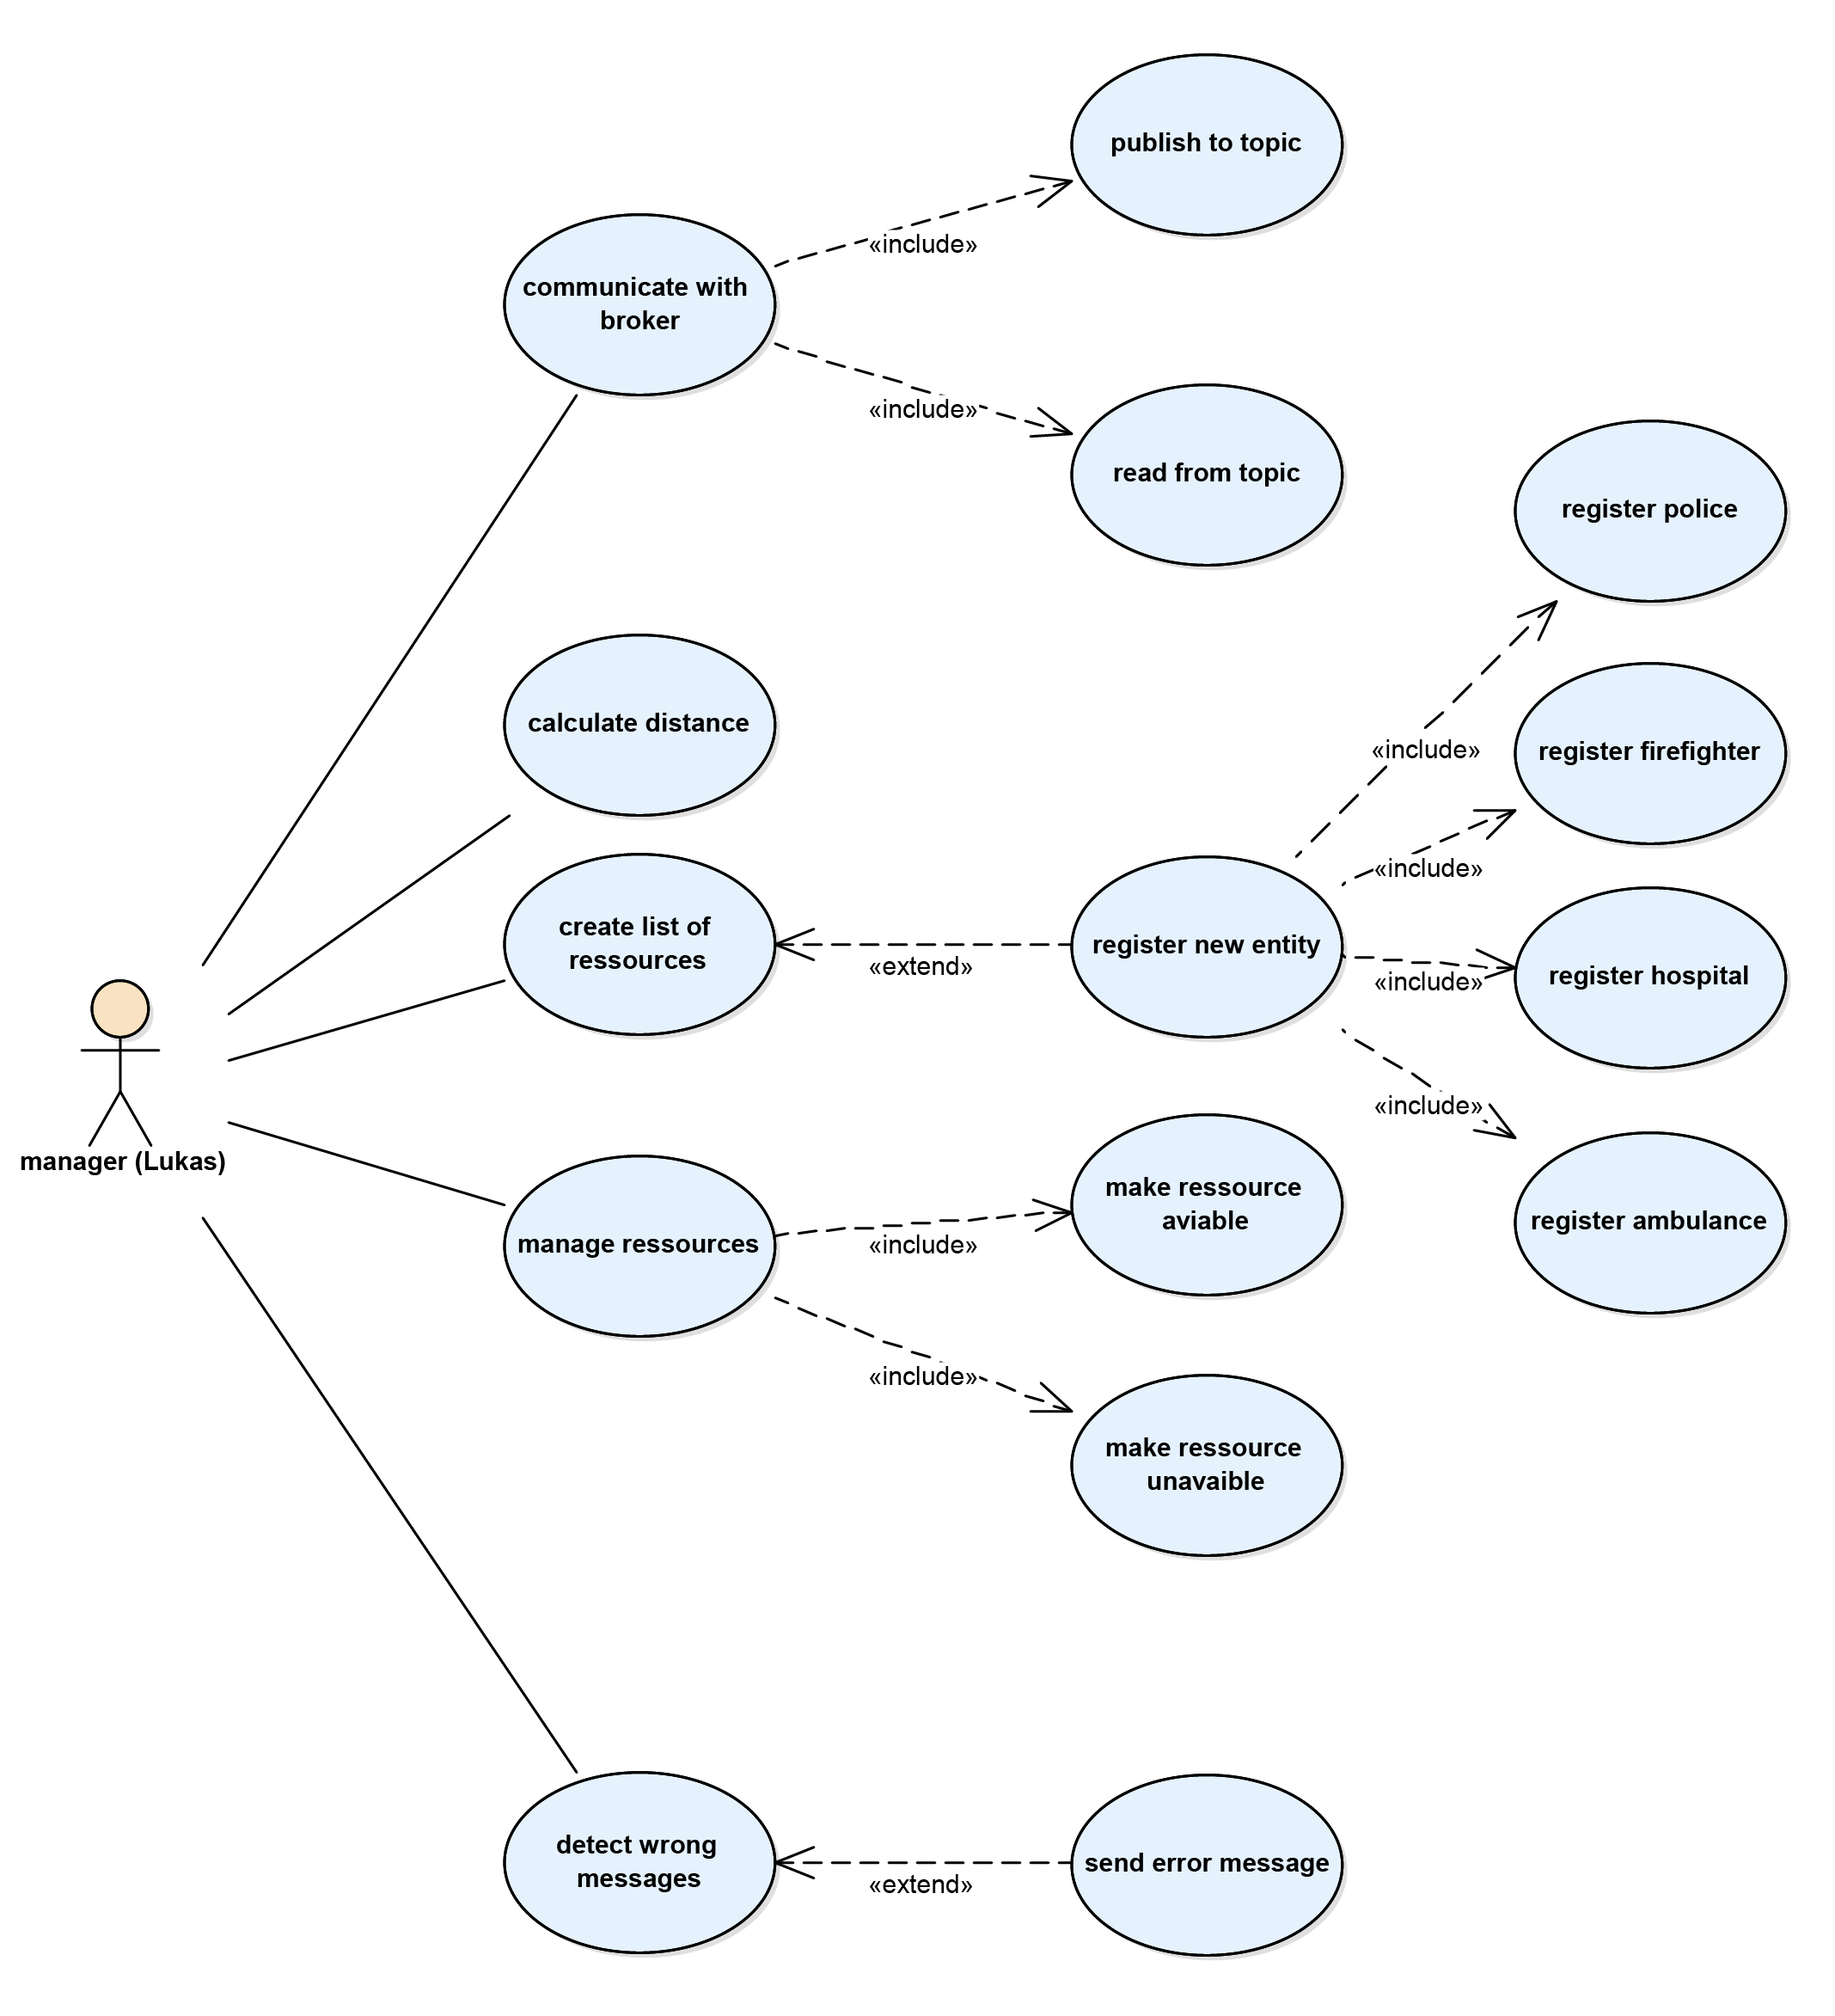
\includegraphics[scale=0.6]{images/walter/usecase_png.png}
\caption{Usecase diagram}
\label{usecase}
\end{figure}

\begin{table}[h]
    \centering
    \begin{tabular}{c|l}
    ID & Requirement  \\
    \hline
    FREQ00 & Communication must take place via defined topics \\
    FREQ01 & The application must be available online \\
    FREQ02 & There must be exception handling \\
    FREQ03 & The application must be able to calculate distances \\
    FREQ04 & The application must keep a list of available resources\\
    FREQ05 & The application must be able to decide depending on the situation \\
    FREQ06 & Wrong requests must have an error message as an answer \\
    \end{tabular}
    \caption{Functional requirements}
    \label{fr}
\end{table}


In addition to the functional requirements there is one non-functional requirement which is shown in table \ref{nfr}.

\begin{table}[h]
    \centering
    \begin{tabular}{c|l}
    ID & Requirement  \\
    \hline
    NFREQ00 & Communication must take place over a protocol \\

    \end{tabular}
    \caption{Non-functional requirements}
    \label{nfr}
\end{table}

The communication is visualized in \ref{SEQ} with the help of a sequence diagram. Communication takes place between the application and the MQTT server. In the upper part of the picture the registration of entities is shown. For example, if an ambulance sends data to the "/hshl/ambulances/" topic, it should be registered. In the lower part of the picture \ref{SEQ}, a case of a user request is visualized. If a user submits a request with a reason, the required assistants should be alerted. In addition, the time until the helpers arrive is transmitted to the user.

\begin{figure}
\sidecaption
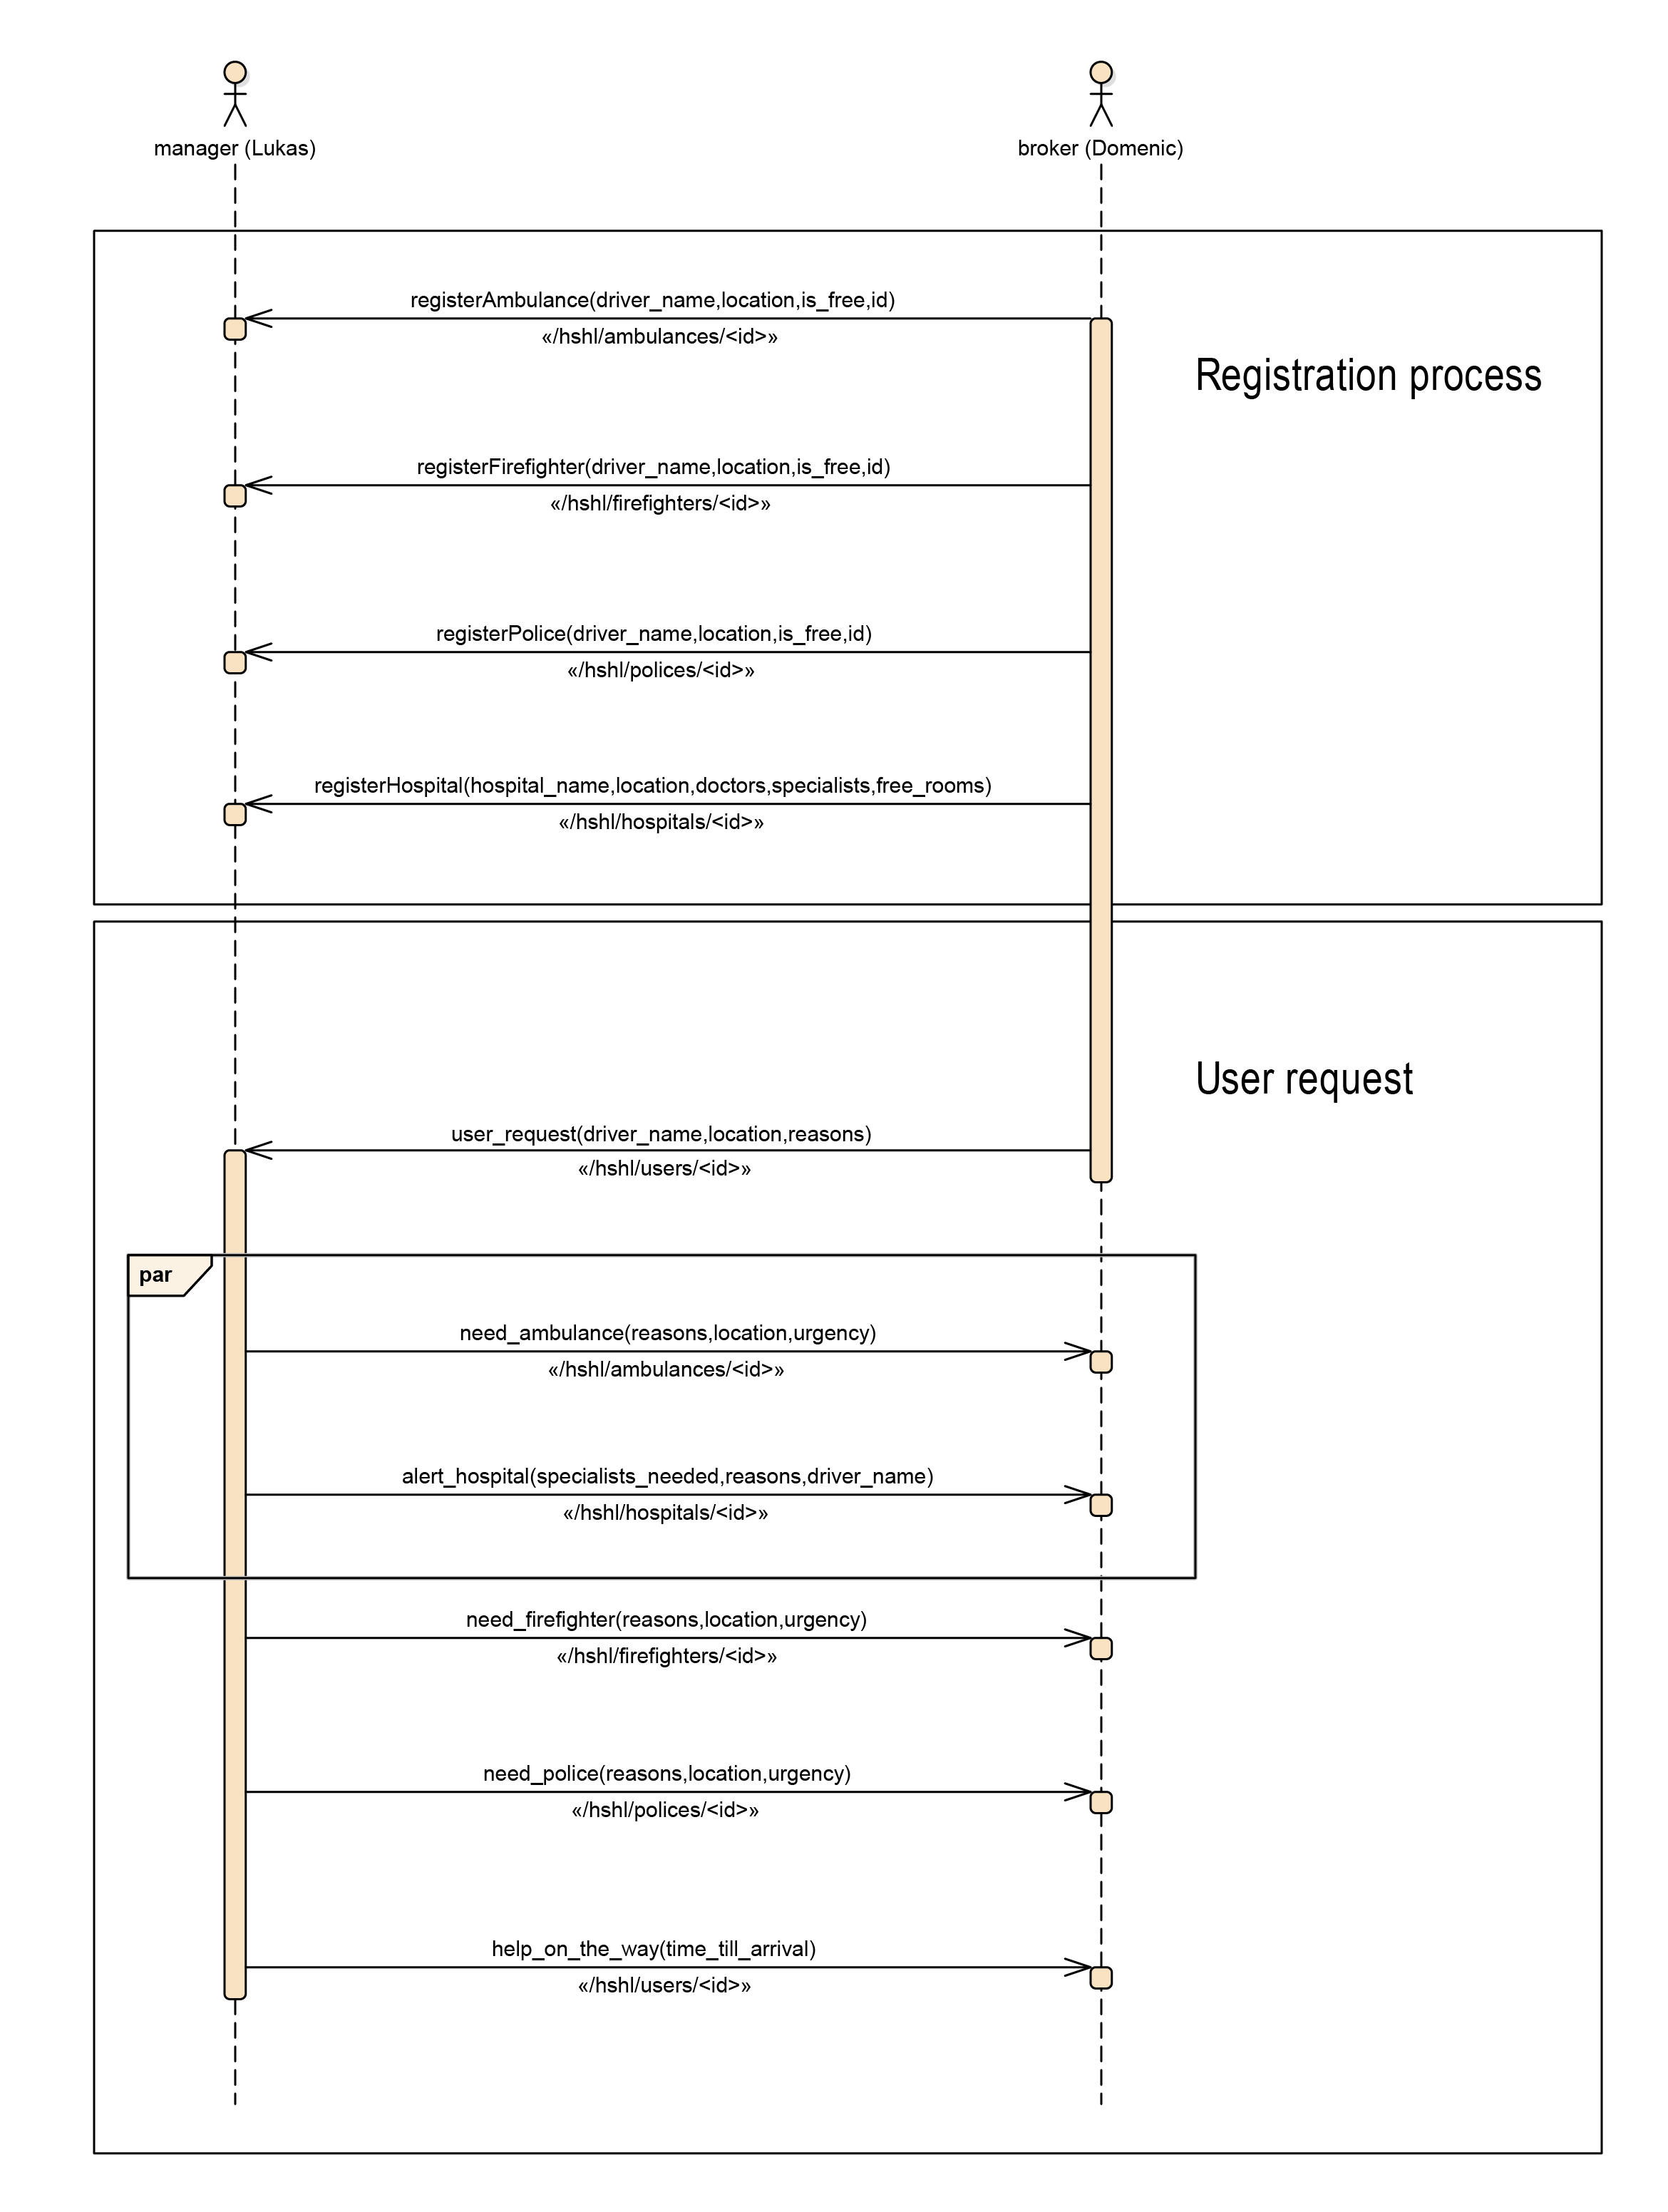
\includegraphics[scale=0.6]{images/walter/sequence_png.png}
\caption{Communication between application and server via MQTT}
\label{SEQ}
\end{figure}



\section{Implementation}
\label{sec:4}

The application was implemented using the programming language python. This language was chosen because a quick and uncomplicated implementation is possible without a lot of fuss. In addition, object-oriented programming is perfect for implementing entities such as different vehicles that can inherit from one another. This behaviour was used, each individual entity is an object with different attributes and different methods. 

The application was versioned with the help of GitHub. Several versions of the software were made available to keep the other project participants up to date. By using GitHub, it was possible to create a documentation for each version with the changes to the previous version and the new functions.

An example of the ambulance class and the basic class everythingThatDrives can be viewed in \ref{entity}. The class ambulance inherits the attributes and methods of everythingThatDrives. In this way, lines can be saved, the code is optimized and easier to understand. The \_\_init\_\_ function is started each time that kind of object is instantiated.

The data was exchanged using the .json format, which stands for JavaScript Object Notation and is a data format. Using this data format, it is possible to extend an existing data set by another variable. Figure \ref{json} shows the form of the data format as it is sent when registering or when updating an entity.

\begin{figure}
\sidecaption
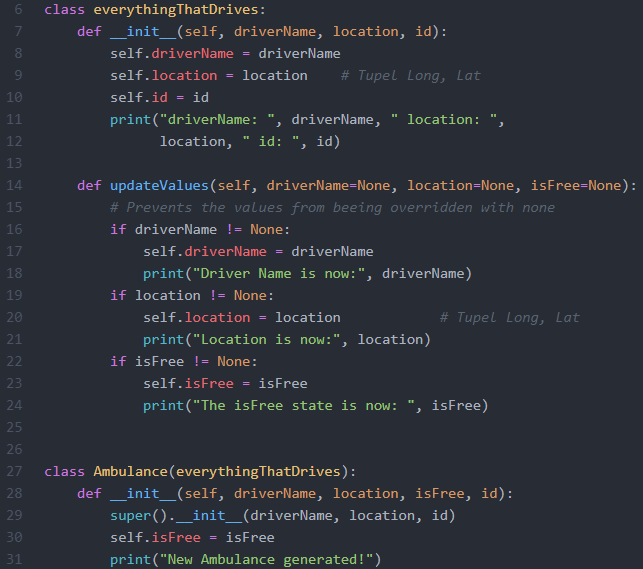
\includegraphics[scale=0.6]{images/walter/code/entity.png}
\caption{The base class everythingThatDrives and the Ambulance class}
\label{entity}
\end{figure}

\begin{figure}
\sidecaption
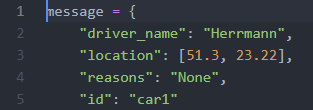
\includegraphics[scale=0.6]{images/walter/code/json.png}
\caption{Data that is sent in .json data format, for example to register or update an ambulance}
\label{json}
\end{figure}

Due to the limited time, not all of the requirements could be met. Requirement FREQ01 and FREQ06 could not be met. All other requirements have been met. The following chapters further explain how the individual requirements were met.


\subsection{FREQ00 - Communication must take place via defined topics}
The FREQ00 requirement was met by the immediate subscription to the main topics when the application was started. This is shown in the code example in graphic \ref{FREQ00}. Line 39 defines the on\_connect() method which is executed the first time the MQTT server is connected. By executing this method, the main topics are subscribed, through which new entities can register. 

The topics under which the entities can receive updates are subscribed at the time the program is running. In line 53 the sub() method is implemented which is responsible for subscribing to new topics if an entity has registered. The try and catch method in line 54 prevents an incorrect user input from causing the program to crash. If a new channel has been subscribed, a message is sent to the corresponding main topic that further communication is now carried out via the new topic.
If an ID is used more than once, this means that a message is sent that this ID already exists and no new topic is subscribed.

\begin{figure}
\sidecaption
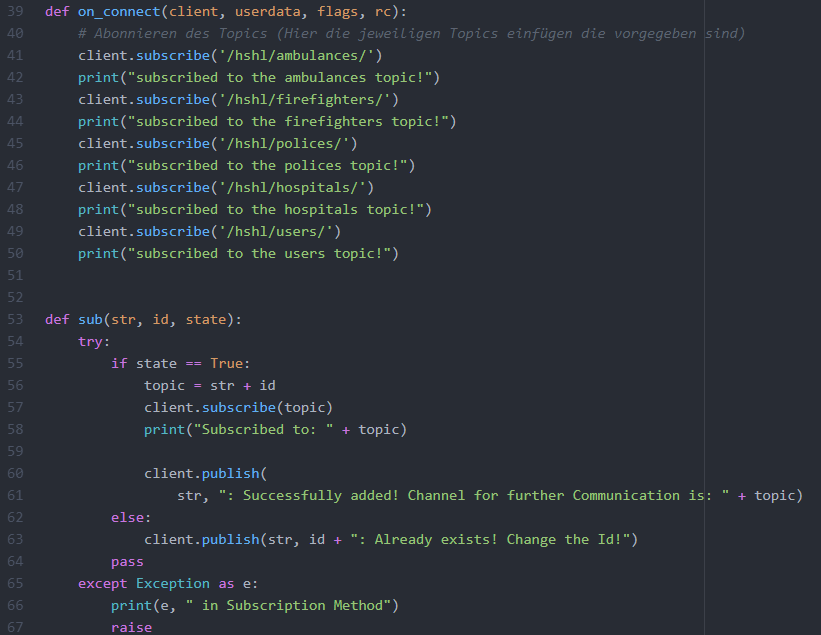
\includegraphics[scale=0.4]{images/walter/code/FREQ00.png}
\caption{Implementation of the requirement FREQ00}
\label{FREQ00}
\end{figure}

\subsection{FREQ02 - There must be exception handling}
FREQ02 was implemented in several places. Exception handling was implemented at every point where an incorrect entry could cause the program to crash. An example of this is shown in the code example in figure \ref{FREQ02}. For example, it is used in the update() method, which is responsible for updating the individual entities, in lines 100, 108 and 117. If an error occurs, it is written to the console.

\begin{figure}
\sidecaption
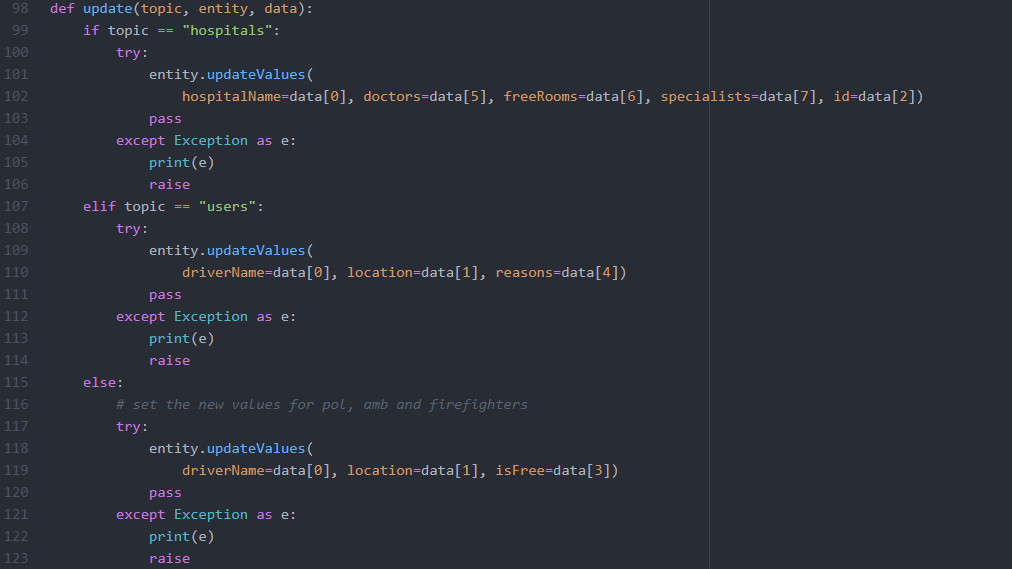
\includegraphics[scale=0.4]{images/walter/code/FREQ02-01.png}
\caption{Implementation of the requirement FREQ02}
\label{FREQ02}
\end{figure}

\subsection{FREQ03 - The application must be able to calculate distances}
The requirement FREQ03 was realized with the help of the GeoPy library. By using this library, the air line between two points on the earth can be calculated very quickly and easily. In line 129 in figure \ref{FREQ03} the corresponding operation is carried out. The geopy.distance.vincenty() function takes two arguments. These are two locations, each with a value for the longitude and one for the latitude. These are given in floating point numbers. The specification .km means that the output is made in kilometres.

\begin{figure}
\sidecaption
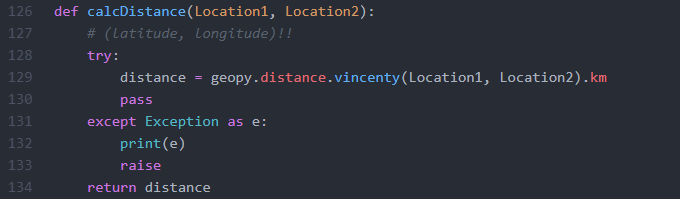
\includegraphics[scale=0.4]{images/walter/code/FREQ02-00.png}
\caption{Implementation of the requirement FREQ03}
\label{FREQ03}
\end{figure}

\subsection{FREQ04 - The application must keep a list of available resources}

At the start of the application, five empty lists are created for the different entities, this can be seen in lines 28 - 32 in figure \ref{FREQ041}. In addition, the so-called allEntityList is created in line 34. This contains all other lists. This has the advantage that if all lists have to be transferred in a function, not every list has to be transferred individually. This has some disadvantages in terms of the performance and the use of resources of the program. However, since these were not decisive factors for this concept, this variant of implementation was chosen. 

The entities are added using the checkNadd() method which is implemented in line 32 in figure \ref{FREQ042}. The method is called as soon as an entity sends a message on one of the main channels. The method then looks to see if the list has a length of zero. If that's is the case, the list is empty and to entity can be added without any further processing. This can be seen in line 33 in Figure \ref{FREQ042}. 

However, if there are already entities in the list, the IDs of all entities are compared with the new one. If the ID already occurs, an error message is sent to the console and the addition of the entity is cancelled. This functionality is implemented in lines 44 - 55 in figure \ref{FREQ042}.


\begin{figure}
\sidecaption
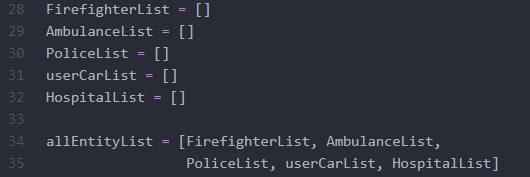
\includegraphics[scale=0.4]{images/walter/code/FREQ04-00.png}
\caption{Implementation of the requirement FREQ04 generating lists}
\label{FREQ041}
\end{figure}

\begin{figure}
\sidecaption
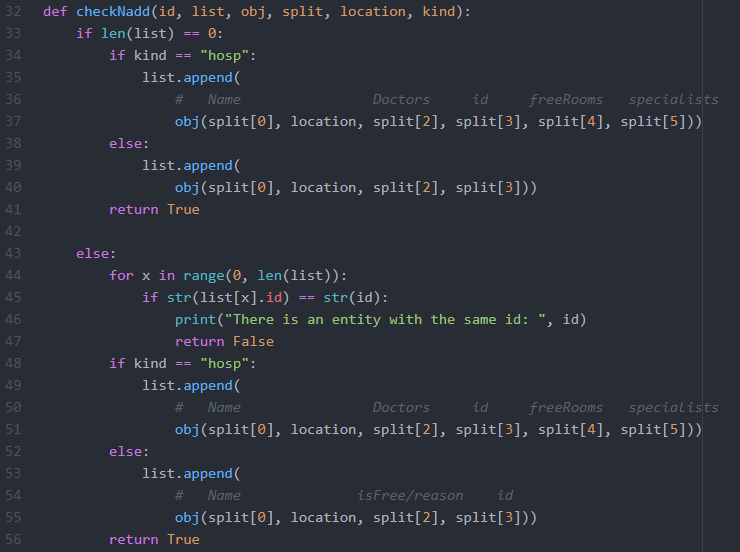
\includegraphics[scale=0.4]{images/walter/code/FREQ04-02.png}
\caption{Implementation of the requirement FREQ04 adding entities to the lists}
\label{FREQ042}
\end{figure}


\subsection{FREQ05 - The application must be able to decide depending on the situation}
Depending on the situation, the application must be able to decide which emergency services are available, which are the closest and which are required. Part of the implementation which only includes the heart\_attack and accident cases can be seen in Figure \ref{decider}. This is done in the decider() method. The decider() method creates an alarm list, which is passed on to the alarm() function to alert emergency vehicles. The alarmList set is created by the getClosest() method. The getClosest() method uses the distance between the user vehicle and the emergency vehicle to select the vehicle with the shortest distance to the user.

\begin{figure}
\sidecaption
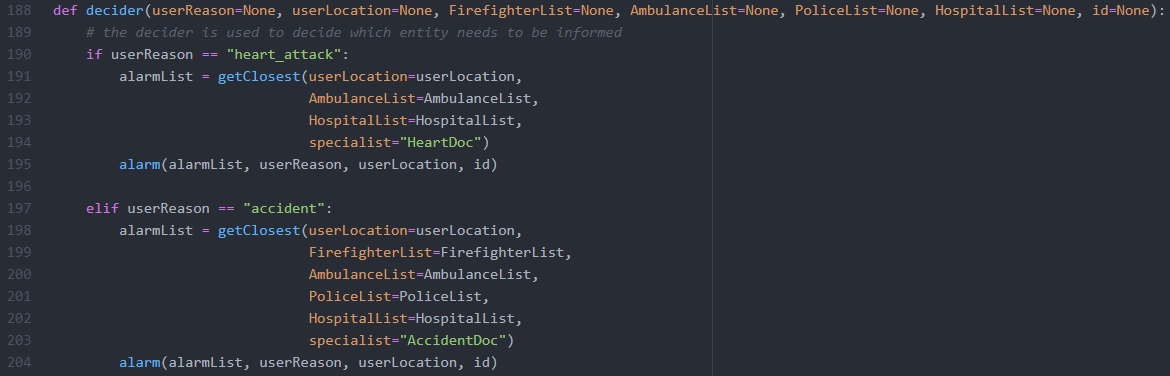
\includegraphics[scale=0.4]{images/walter/code/decider.png}
\caption{Implementation of the requirement FREQ05}
\label{decider}
\end{figure}


\subsection{NFREQ00 - Communication must take place over a protocol}
The non-functional requirement that communication must take place via a protocol is met by using the MQTT protocol. MQTT is implemented with the help of the paho-MQTT library.

\section{Results}
\label{sec:5}
Registering and updating emergency vehicles as well as hospitals and user vehicles works as it should. In addition, the calculation of the distance and the situation-related alarming of the service vehicles is functional. Only two of the requirements, the application should be available online and incorrect requests must have an error message as an answer could either not be implemented completely or not at all.

A program sequence is shown in \ref{console}. At the beginning, the main topics are subscribed. Then different entities are created one after another, starting with a user vehicle followed by a firefighter, a police car, an ambulance and a hospital.

\begin{figure}
\sidecaption
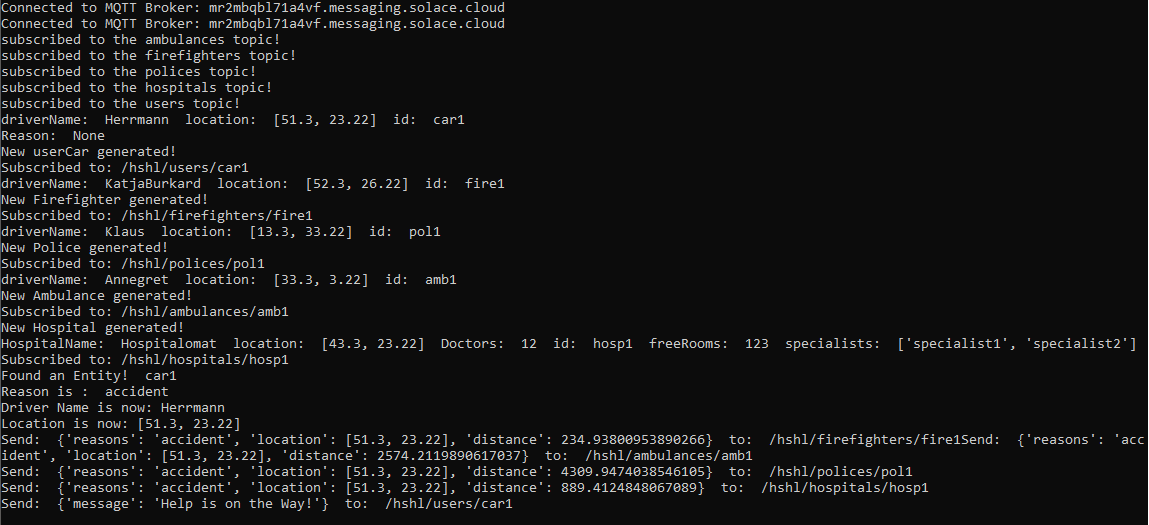
\includegraphics[scale=0.5]{images/walter/console.PNG}
\caption{Program sequence with test data}
\label{console}
\end{figure}
After the entities have been registered, the user car sends an update. The update contains the reason accident. With this reason, the decider method is called which immediately alerts the nearest emergency vehicles and the hospital. The user receives the message that help is on the way.

In the last version of the application it is not possible to decide which hospital will be alerted based on the specialists working in a hospital. In this case it is always assumed that every specialist is available in every hospital. In addition, the number of free beds in the hospital is not considered.

The code is sometimes difficult to understand due to many nested methods that are not often adequately documented. This complex nesting probably has the consequence that in practice the program ran into different deadlocks with the other project participants.

The program sometimes behaves in an unpredictable way, for example, if a lot of data is received at once, errors can occur. This could be remedied by using threading. Each entity could have its own application that monitors the entity. However, this would greatly increase the power consumption of the application and add other complex structures. 

Improvements in the use of resources can be made in many places. For example, some redundant pieces of code could be outsourced in functions.

The biggest challenge in this project was communicating with the other project participants. It was not always clear where the problems were, which greatly delayed the development process. One solution to this problem would be to use Slack. In previous projects, this application has greatly improved collaboration in groups.


\section{Conclusion}
\label{sec:5}
The application works perfectly with test data. The requirements that were not met could simply be implemented in future versions. It could also be implemented that, depending on which specialist works in a hospital, it is decided which hospital is more suitable for the user. The number of free beds should also be considered. It would be conceivable not to calculate the air line of the distance but the actual distance when using the streets.

The general stability of the application could be greatly improved by better documenting the code and thus easier understanding, which makes finding errors easier.

By using .json, the expansion of the program by other factors such as the current heart rate of the users is very easy. These options offer almost endless possibilities for expansion. For example, a hospital and an ambulance could be given a warning before a heart attack occurs and thus potentially save lives.

\newpage
\bibliographystyle{IEEEtran}
\bibliography{chapters/chapter2_lucas_w/chapter.bib}
